\documentclass{template/openetcs_article}

\usepackage[english]{babel}
\usepackage{amsmath}
\usepackage{amssymb,amsfonts,textcomp}
\usepackage{array}
\usepackage{supertabular}
\usepackage{hhline}
\usepackage{graphicx}
\usepackage{lscape}
\usepackage{float}
\usepackage{url}
\usepackage{hyperref}
\usepackage{breakurl}
\usepackage[titletoc]{appendix}
\usepackage{lipsum}
\makeatletter
\newcommand\arraybslash{\let\\\@arraycr}
\makeatother
\setlength\tabcolsep{1mm}
\renewcommand\arraystretch{1.3}
\newcounter{Ilustracin}
\renewcommand\theIlustracin{\arabic{Ilustracin}}
\title{openETCS}

\DeclareGraphicsExtensions{.pdf,.png,.jpg}
\usepackage{float}
\restylefloat{figure}

\definecolor{grey}{rgb}{0.8,0.8,0.8}
\definecolor{lightgrey}{rgb}{0.95,0.95,0.95}

\usepackage{hhline}
\usepackage{booktabs}
\usepackage{multirow}
\usepackage{color, colortbl}
\definecolor{myblue}{rgb}{0.6,.6,1}
\definecolor{mydarkblue}{rgb}{0,0,0.5}
\definecolor{mylightblue}{rgb}{0.8,0.8,1}
\definecolor{grey}{rgb}{0.8,0.8,0.8}
\definecolor{lightgrey}{rgb}{0.95,0.95,0.95}
\usepackage{hyperref}
\hypersetup{colorlinks=true, linkcolor=mydarkblue, urlcolor=mydarkblue}




%%%%% comments %%%%%
% To allow MS Word style comments at the document margin we use the todonotes package. A comment is made as follows:

%\mycomment[IN]{text}

% The text in brackets should be your initials and the text in curly braces is your actual comment. Comments are numbered automatically. 
\usepackage[textwidth=2.7cm,textsize=scriptsize,linecolor=green!40,backgroundcolor=green!40]{todonotes}
\usepackage{hyperref}


\newcounter{mycommentcounter}
\newcommand{\mycomment}[2][]
{
\refstepcounter{mycommentcounter}%
\todo[color={red!100!green!33}]{
\textbf{[\uppercase{#1} \themycommentcounter]:} #2}
}





\graphicspath{{./template/}{.}{./images/}}
\begin{document}
\frontmatter
\project{openETCS}

%Please do not change anything above this line
%============================
% The document metadata is defined below

%assign a report number here
\reportnum{OETCS/WP1/D1.3}

%define your workpackage here
\wp{Work-Package 1: ``Management''}

%set a title here
\title{Software Configuration Management Plan}

%set a subtitle here
\subtitle{DRAFT}

%set the date of the report here
\date{\today}

%define a list of authors and their affiliation here

\author{Jürgen Weiss}

\affiliation{ALSTOM Transport Deutschland GmbH\\
  Friedrichstrasse 149 \\
  10117 Berlin, Germany}

\author{Peer Jacobsen}

\affiliation{ALSTOM Transport Deutschland GmbH\\
  Friedrichstrasse 149 \\
  10117 Berlin, Germany}

% define the coverart
\coverart[width=350pt]{openETCS_EUPL}

%define the type of report
\reporttype{Description of work}




%=============================
%Do not change the next three lines
\maketitle
\tableofcontents
\listoffiguresandtables
\newpage
%=============================

% The actual document starts below this line
%=============================


%Start here

%\begin{document}

\section*{Document History}
\label{sec:Document History}

\begin{center}
\begin{longtable}{m{1.5cm}m{2cm}m{2cm}m{4.5cm}m{4cm}}
\caption{Document history}\\

\hline \rowcolor{lightgrey} \multicolumn{1}{l}{Version} & \multicolumn{1}{l}{Date} & \multicolumn{1}{l}{Chapters modified} & \multicolumn{1}{l}{Reason} & \multicolumn{1}{l}{Name} \\ \hline
\endfirsthead

\multicolumn{5}{c}%
{{\bfseries \tablename\ \thetable{} -- continued from previous page}} \\
\hline \rowcolor{lightgrey} \multicolumn{1}{l}{Version} & \multicolumn{1}{l}{Date} & \multicolumn{1}{l}{Chapters modified} & \multicolumn{1}{l}{Reason} & \multicolumn{1}{l}{Name} \\ \hline
\endhead

\hline \hline
\endlastfoot

0.0.0 & 09/08/2013 & All New & Frame and Basics definition & Jürgen Weiss (ALSTOM)\\\hline
0.0.1 & 13/02/2014 & All & Changed structure and content to comply with IEEE Std 828-2005 & Peer Jacobsen (ALSTOM)\\\hline
\end{longtable}
\end{center}

\newpage


\section{Introduction} % Section 1
\label{sec:Introduction}

This chapter introduces the concept of Software Configuration Management (SCM), describes the purpose and scope of this document and defines references, guidelines and standards as well as key terms, abbreviations and acronyms.


\subsection{Purpose} % Subsection 1.1
\label{sec:Purpose}

This document is the Software Configuration Management Plan (SCMP) for the openETCS project. It defines the methods and tools to identify and control the software and its functional attributes throughout its development and use. It also documents how and when these methods and tools are to be used, states who is responsible, and specifies the required resources.

The overall purpose is to maintain software integrity and configuration traceability during the entire software life cycle (including development as well as maintenance). The intended audience of the SCMP are persons involved in or responsible for this process. Roles and responsibilities as well as respective activities are defined or referred to in the corresponding sections of this SCMP (see sections \ref{sec:Responsibilities} and \ref{sec:SCM Activities}).


\subsection{Scope } %Subsection 1.2
\label {sec:Scope}

This SCMP applies to the entire life cycle of critical software as well as to noncritical software and software already developed within the context of the openETCS project. It provides technical and supervising direction to ensure that SCM activities are successfully implemented for the openETCS project.

SCM includes the following activities:

\vspace{-10pt}
\begin{itemize}
\item Identification and definition of configuration items and baselines.
\item Review, approval, and control of changes.
\item Tracking and reporting of changes.
\item Audits and reviews of the software product in development.
\item Control of interface documentation.
\item Management of software release and delivery activities.
\end{itemize}

To provide all necessary information, the SCMP is structured into the following parts:

\textcolor{red}{Note: This is the structure given in IEEE 828-2005.}

\vspace{-10pt}
\begin{itemize}
\item Introduction: Describes the purpose and scope of the SCMP. Also lists reference documents, guidelines and standards as well as key terms, abbreviations and acronyms.
\item SCM Management (see section \ref{sec:SCM Management}): Describes authorities and responsibilities related to managing and implementing SCM activities (i.e. who).
\item SCM Activities (see section \ref{sec:SCM Activities}): Describes the SCM activities required for the openETCS project (i.e. what).
\item SCM Schedules (see section \ref{sec:SCM Schedules}): Describes the coordination of SCM activities with other activities within the openETCS project (i.e. when).
\item SCM Resources (see section \ref{sec:SCM Resources}): Describes tools as well as physical and human resources required for SCM activities (i.e. how).
\item SCMP Maintenance (see section \ref{sec:SCMP Maintenance}): Describes how the SCMP will be updated while in effect.
\end{itemize}


\subsection{References, Guidelines and Standards} % Subsection 1.3
\label {sec:References, Guidelines and Standards}

In general, the references, guidelines and standards listed in the Project Quality Assurance Plan (QA Plan) also apply to the SCMP (see QA Plan section 1.5). This section of the SCMP only lists references, guidelines and standards that specifically apply to the SCMP and are not listed in the QA Plan. 


\subsubsection{References} % Subsection 1.3.1
\label{sec:References}

The following table lists reference documents that provide additional information relevant to the SCMP:

\begin{center}
\begin{longtable}{m{1.5cm}m{6.5cm}m{1.5cm}m{2cm}m{2.5cm}}
\caption{References}\\

\hline \rowcolor{lightgrey} \multicolumn{1}{l}{Internal Code} & \multicolumn{1}{l}{Name} & \multicolumn{1}{l}{Version/ Edition/ Date} & \multicolumn{1}{l}{Repository} & \multicolumn{1}{l}{Responsible} \\ \hline
\endfirsthead

\multicolumn{5}{c}%
{{\bfseries \tablename\ \thetable{} -- continued from previous page}} \\
\hline \rowcolor{lightgrey} \multicolumn{1}{l}{Internal Code} & \multicolumn{1}{l}{Name} & \multicolumn{1}{l}{Version/ Edition/ Date} & \multicolumn{1}{l}{Repository} & \multicolumn{1}{l}{Responsible} \\ \hline
\endhead

\hline \hline
\endlastfoot

\cite{QAP} & Quality Assurance Plan & \centering 0.10.6 & governance & QA Manager\\\hline
\cite{CMP} & Change/Problem Management Process & \centering 0.1.0 & governance & QA Manager\\\hline
\cite{FPP} & Full Project Proposal & \centering 3.0.2 & management & n/a\\\hline
\cite{RDP} & Software Release and Deployment Plan & \centering n/a & n/a & n/a\\\hline
\end{longtable}
\end{center}

\textcolor{red}{Open: Figure out how to add break in table header. Fill gaps. Additional relevant docs?}


\subsubsection{Guidelines} % Subsection 1.3.2
\label{sec:Guidelines}

The following table lists guidelines that have been followed in the creation of the SCMP:

\begin{center}
\begin{longtable}{m{1.5cm}m{6.5cm}m{1.5cm}m{2cm}m{2.5cm}|}
\caption{Guidelines}\\

\hline \rowcolor{lightgrey} \multicolumn{1}{l}{Internal Code} & \multicolumn{1}{l}{Name} & \multicolumn{1}{l}{Version/ Edition/ Date} & \multicolumn{1}{l}{Repository} & \multicolumn{1}{l}{Responsible} \\ \hline
\endfirsthead

\multicolumn{5}{c}%
{{\bfseries \tablename\ \thetable{} -- continued from previous page}} \\
\hline \rowcolor{lightgrey} \multicolumn{1}{l}{Internal Code} & \multicolumn{1}{l}{Name} & \multicolumn{1}{l}{Version/ Edition/ Date} & \multicolumn{1}{l}{Repository} & \multicolumn{1}{l}{Responsible} \\ \hline
\endhead

\hline \hline
\endlastfoot

\cite{IEEE828} & IEEE Std 828 - Standard for Software Con-figuration Management Plans &
\centering IEEE STD 828-2005 & n/a & n/a\\\hline
\end{longtable}
\end{center}


\subsubsection{Standards} % Subsection 1.3.2
\label{sec:Standards}

There are no standards that apply specifically to the SCMP. Standards that apply to the entire openETCS project are listed in the QA Plan (see QA Plan section 1.5).


\subsection{Key Terms, Abbreviations and Acronyms} % Subsection 1.4
\label{sec:Key Terms, Abbreviations and Acronyms}

A central glossary is part of the openETCS project (see QA Plan section 1.6.1).  The following sections only list important key terms, abbreviations and acronyms that are used in this SCMP.

\textcolor{red}{Open: Not sure what to refer to here. Do we have a central glossary yet?}


\subsubsection{Key Terms} % Subsection 1.4.1
\label{sec:Key Terms}

The following table provides descriptions or explanations for key terms that are used in this SCMP:

\textcolor{red}{Open: Fill when content of doc is fixed/final.}

\begin{center}
\begin{longtable}{m{4cm}m{10cm}|}
\caption{Key terms}\\

\hline \rowcolor{lightgrey} \multicolumn{1}{l}{Term} & \multicolumn{1}{l}{Meaning} \\ \hline
\endfirsthead

\multicolumn{2}{c}%
{{\bfseries \tablename\ \thetable{} -- continued from previous page}} \\
\hline \rowcolor{lightgrey} \multicolumn{1}{l}{Term} & \multicolumn{1}{l}{Meaning} \\ \hline
\endhead

\hline \hline
\endlastfoot

 & \\\hline
 & \\\hline
\end{longtable}
\end{center}


\subsubsection{Abbreviations and Acronyms} % Subsection 1.4.2
\label{sec:Abbreviations and Acronyms}

The following table lists abbreviations and acronyms used in this SCMP:

\textcolor{red}{Open: Review when content of doc is fixed/final.}

\begin{center}
\begin{longtable}{m{4cm}m{10cm}|}
\caption{Abbreviations and acronyms}\\

\hline \rowcolor{lightgrey} \multicolumn{1}{l}{Abbreviation/Acronym} & \multicolumn{1}{l}{Meaning} \\ \hline
\endfirsthead

\multicolumn{2}{c}%
{{\bfseries \tablename\ \thetable{} -- continued from previous page}} \\
\hline \rowcolor{lightgrey} \multicolumn{1}{l}{Abbreviation/Acronym} & \multicolumn{1}{l}{Meaning} \\ \hline
\endhead

\hline \hline
\endlastfoot

CI & Configuration Item\\\hline
CSA & Configuration Status Accounting\\\hline
ETCS & European Train Control System\\\hline
FCA & Functional Configuration Audit\\\hline
FPP & Full Project Proposal\\\hline
n/a & Not applicable\\\hline
PCA & Physical Configuration Audit\\\hline
QA Plan	& Project Quality Assurance Plan\\\hline
SCM & Software Configuration Management\\\hline
SCMP & Software Configuration Management Plan\\\hline
SRS & System Requirements Specification\\\hline
V \& V & Verification and Validation\\\hline
WP & Work Package\\\hline
\end{longtable}
\end{center}

\newpage


\section{SCM Management} % Section 2
\label{sec:SCM Management}

This chapter describes the allocation and management of authority and responsibility regarding the SCM activities for the openETCS project.


\subsection{Organization} % Subsection 2.1
\label{sec:Organization}

The following table provides the organizational units that participate in or are responsible for SCM activities within the openETCS project:

\textcolor{red}{Open: Not sure if it makes sense to list the WPs. Review once activities etc. are defined.}

\begin{center}
\begin{longtable}{m{4cm}m{10cm}|}
\caption{Organization}\\

\hline \rowcolor{lightgrey} \multicolumn{1}{l}{Organizational Unit} & \multicolumn{1}{l}{Role in Project Structure} \\ \hline
\endfirsthead

\multicolumn{2}{c}%
{{\bfseries \tablename\ \thetable{} -- continued from previous page}} \\
\hline \rowcolor{lightgrey} \multicolumn{1}{l}{Organizational Unit} & \multicolumn{1}{l}{Role in Project Structure} \\ \hline
\endhead

\hline \hline
\endlastfoot

WP1 Project Management & Project management and governance\\\hline
WP2 Requirements for Open Proofs & Define requirements for modeling, verification and validation process.\\\hline
WP3 Modeling - Code Generation & Provide the formal model and the source code by using the tool chain.\\\hline
WP4 Validation \& Verification Strategy & Validation and verification of the model.\\\hline
WP5 openETCS Demonstrator & Provide the means to show the results of the project.\\\hline
WP6 Dissemination, Exploitation and Standardization & Organize the market, exploitation, dissemination and standardization activities.\\\hline
WP7 Toolchain & Provide the tool chain for design, development, verification and validation.\\\hline
\end{longtable}
\end{center}

The openETCS project structure is described in more detail in the QA Plan (see QA Plan chapter 2). The individual work packages are described in detail in the Full Project Proposal (see FPP chapter 5).


\subsection{Responsibilities} % Subsection 2.2
\label{sec:Responsibilities}

The following table matches responsibilities for the individual SCM activities that have been defined for the openETCS project (see chapter \ref{sec:SCM Activities}) to organizational units or specific positions:

\textcolor{red}{Open: Review once activities etc. are defined. Match to organizational units.}

\begin{center}
\begin{longtable}{m{10cm}m{4cm}|}
\caption{Responsibilities}\\

\hline \rowcolor{lightgrey} \multicolumn{1}{l}{SCM Activity} & \multicolumn{1}{l}{Responsible} \\ \hline
\endfirsthead

\multicolumn{2}{c}%
{{\bfseries \tablename\ \thetable{} -- continued from previous page}} \\
\hline \rowcolor{lightgrey} \multicolumn{1}{l}{SCM Activity} & \multicolumn{1}{l}{Responsible} \\ \hline
\endhead

\hline \hline
\endlastfoot

Responsible for monitoring that the SCMP is implemented and followed.

Select and approve CIs and baselines. & QA Manager (WP1 Task Leader/Project Leader QA)\\\hline
System configuration owner and responsible for the SCMP.

Select and approve CIs and baselines. & Configuration Manager\\\hline
Initiate CI identification and selection process in work package.

Select and approve CIs and baselines. & Work Package Leader\\\hline
Responsible for monitoring content and implementation of the SCMP. & Assessor\\\hline
Responsible for ensuring that software and derived specifications and requirements are under system configuration and change management control. & Requirement Manager\\\hline
Responsible for ensuring that the design documents are under system configuration and change management control. & Designer\\\hline
Responsible for maintaining the generated or modified data/codes/models under system configuration and change management control. & Implementer\\\hline
\end{longtable}
\end{center}

The individual roles are described in more detail in the QA Plan (see QA Plan Appendices CAT1 to CAT 3).


\subsection{Applicable Policies, Directives and Procedures} % Subsection 2.3
\label{sec:Applicable Policies, Directives and Procedures}

As the organizational unit responsible for Quality Assurance, WP1 is responsible for the overall SCM process. Within WP1, the role Quality Assurance Manager is responsible for implementation of the SCMP and corresponding SCM activities as well as identification, assessment and management of risks related to SCM activities.

In addition, the role Configuration Manager is responsible for the content of the SCMP, the definition of SCM activities and the content of the Configuration Item Register.

Independent monitoring as well as independent identification and assessment of risks related to SCM activities is the responsibility of the role Assessor.

\textcolor{red}{Open: Org unit for Assessor?}

\newpage


\section{SCM Activities} % Section 3
\label{sec:SCM Activities}

This chapter describes the functions and tasks that are necessary to manage the configuration of the software system. It includes technical as well management-related SCM activities that are grouped as follows:

\vspace{-10pt}
\begin{itemize}
\item Configuration item identification
\item Baseline identification
\item Configuration control
\item Configuration status accounting
\item Configuration evaluation and review
\item Interface control
\item Release management and delivery
\end{itemize}

The following figure gives an overview of how these SCM activities function together:

\begin{figure}[H]
\centering
\caption{Overview of SCM activities}
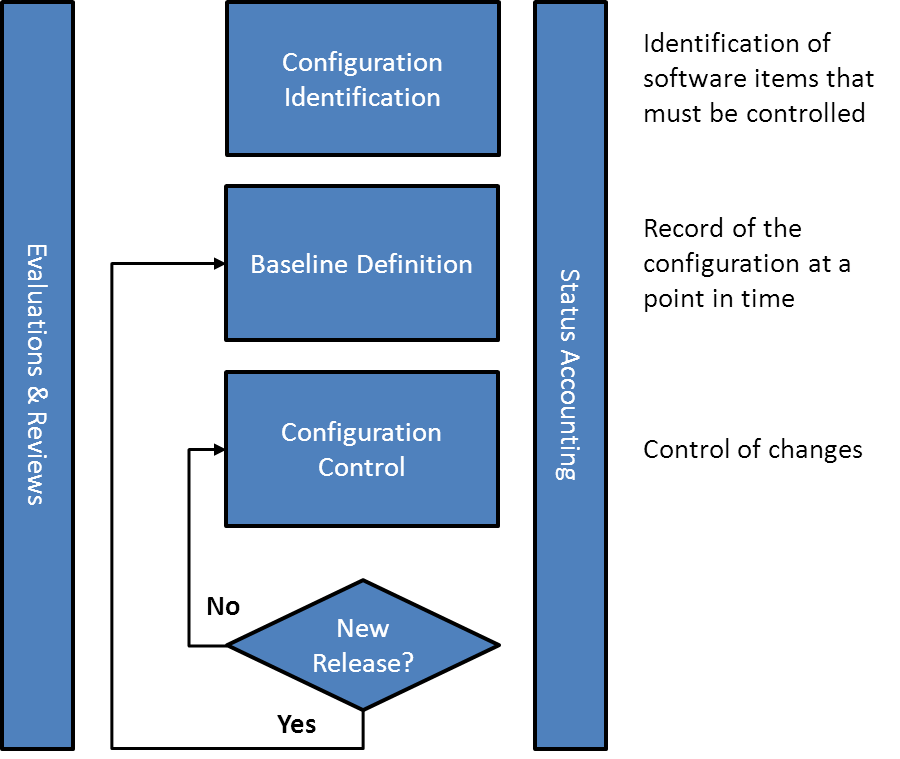
\includegraphics[scale=0.8]{./Figure/SCM_Overview.png}
\end{figure}


\subsection{Configuration Item Identification} % Subsection 3.1
\label{sec:Configuration Item Identification}

Configuration identification establishes and maintains the definitive basis for configuration control of a system and its configuration items (CIs). It defines how CIs are selected, grouped, classified and defined by physical and functional characteristics. The goal is to ensure that all relevant CIs are properly identified, documented and tracked throughout their life cycle.

A CI is an entity that is subject to configuration control. CIs differ in complexity, size and type and encompass both the output of the development process (e.g. code, databases, test plans) as well as elements of the support environment (e.g. compilers, programming tools, test beds).

\textcolor{red}{Open: Not sure if the above is right. Maybe we only want to control CIs that are part of a baseline?}

In a complex system such as the openETCS software, CIs are structured hierarchically, meaning that complex high level or so-called aggregate CIs can be subdivided into several subordinate CIs that are easier to document and control. Because it is formed of several CIs, an aggregate CI can be very similar to a baseline. The key difference is that an aggregate CI is a logical and/or convenient grouping of CIs, whereas a baseline represents a deliverable (see also section \ref{sec:Baseline Identification}).

The following figure provides an example of CIs in a signalling system:

\begin{figure}[H]
\centering
\caption{Signalling system CI example}
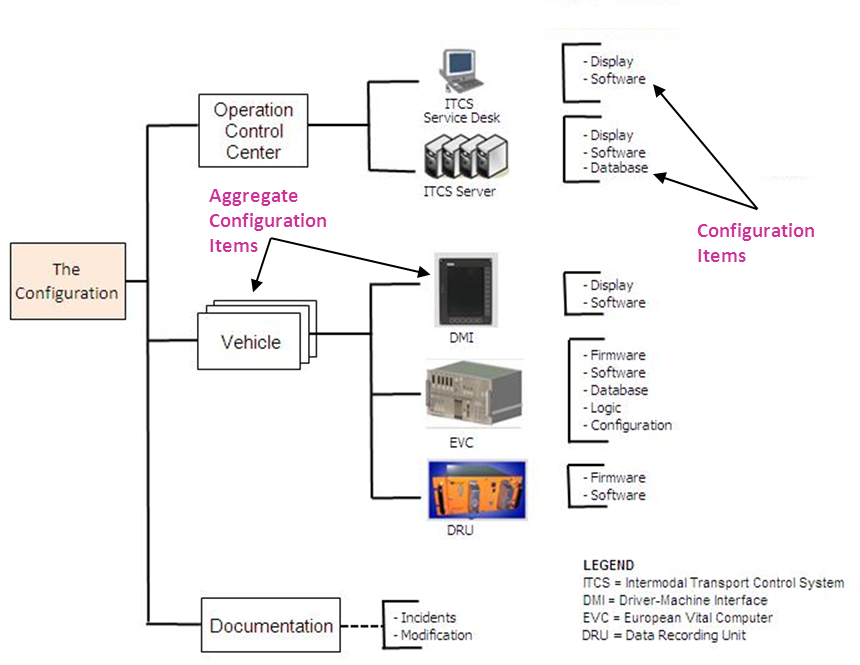
\includegraphics[scale=1.0]{./Figure/CI_Example.png}
\end{figure}

The following sections describe how CIs are identified and managed in the openETCS project.


\subsubsection{CI Identification and Selection Process} % Subsection 3.1.1
\label{sec:CI Identification and Selection Process}

The identification and selection of CIs is an ongoing process that relies on the judgment and recommendations of people involved at all levels of the openETCS project. In most cases, the process will begin in the Scrum Teams of the individual work packages of the openETCS project.
The following figure gives a general overview of the CI identification and selection process:

\begin{figure}[H]
\centering
\caption{CI identification and selection process}
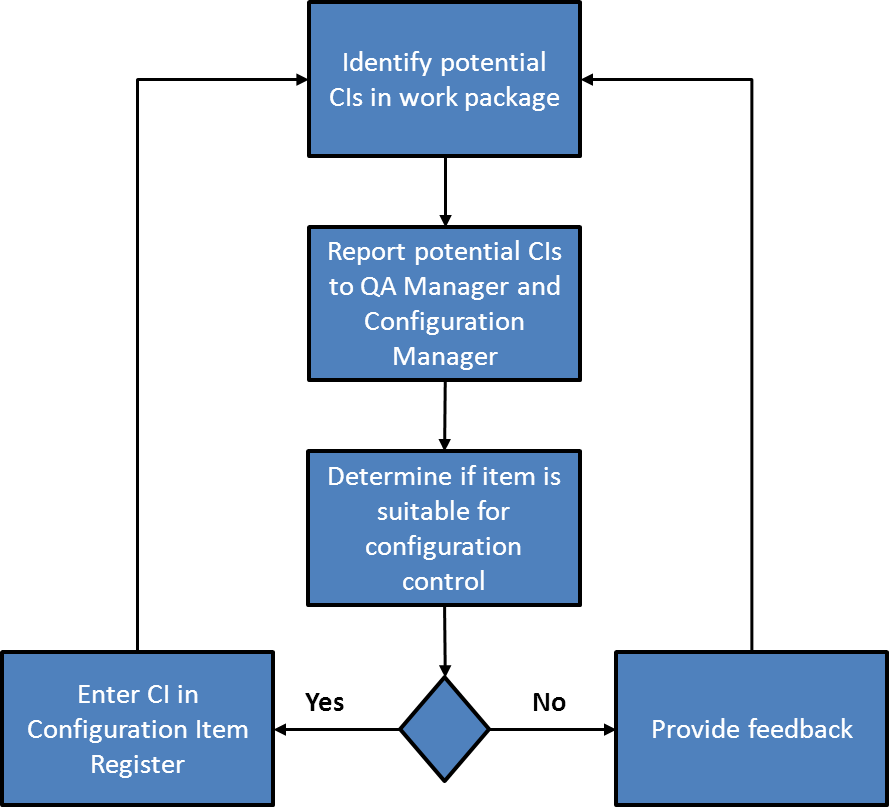
\includegraphics[scale=1.0]{./Figure/CI_Process.png}
\end{figure}

Process description:

\vspace{-10pt}
\begin{enumerate}
\item Work Package Leaders are responsible for starting and supervising the identification and selection of potential CIs in their WP. The identification and selection itself should involve people who are close to the subject matter (e.g. Scrum Teams). Criteria and a checklist for identifying potential CIs are provided in section \ref{sec:CI Identification and Selection Criteria}.
\item Potential CIs are reported to the QA Manager and the Configuration Manager.
\item QA Manager and Configuration Manager provide feedback regarding the suitability of the potential CI for configuration control. They also coordinate the decision process with the involved persons in the WP that has proposed the CI.
\item If the CI is suitable for configuration control, the Configuration Manager enters it in the Configuration Item Register. Attributes that must be provided for each CI are given in section \ref{sec:CI Attributes}.
\end{enumerate}

\textcolor{red}{Open: Define CI Register. Where are we planning to enter and maintain CI information?}


\subsubsection{CI Identification and Selection Criteria} % Subsection 3.1.2
\label{sec:CI Identification and Selection Criteria}

The following general criteria can be used as a guideline when identifying and selecting CIs:

\vspace{-10pt}
\begin{itemize}
\item Designating a component as a CI increases its visibility and control within the project. This is essential for system critical or high risk components.
\item Major functional design components should be designated as (aggregate) CIs. These components form a good starting point for the initial selection.
\item Complex (aggregate) CIs can be subdivided into individual CIs. This will likely happen during the design and development phases. Subordinate CIs should be functionally interrelated.
\item High level (aggregate) CIs should be separable entities that implement at least one function.
\item Operational software and support software should be differentiated as separate CIs.
\item Selecting a large number of CIs can lead to delays and increase costs.
\item Selecting very few CIs can mean that the individual CIs are unnecessarily complex and difficult to document and control. 
\end{itemize}

The following table can be used as a checklist to determine if an item should be designated as a CI (if there are more “yes” answers than “no” answers, it should probably be a CI):

\begin{center}
\begin{longtable}{m{12cm}m{1cm}m{1cm}}
\caption{CI checklist}\\

\hline \rowcolor{lightgrey} \multicolumn{1}{l}{Question} & \multicolumn{1}{l}{Yes} & \multicolumn{1}{l}{No} \\ \hline
\endfirsthead

\multicolumn{3}{c}%
{{\bfseries \tablename\ \thetable{} -- continued from previous page}} \\
\hline \rowcolor{lightgrey} \multicolumn{1}{l}{Question} & \multicolumn{1}{l}{Yes} & \multicolumn{1}{l}{No} \\ \hline
\endhead

\hline \hline
\endlastfoot

Is the item critical or high risk? Does failure of the item have a significant impact? & &\\\hline
Does the item implement critical functionality (e.g. collision avoidance)? Would control and verification of the functionality be increased by CI status? & &\\\hline
Does the item require changes in design or development? & &\\\hline
Is the item computer hardware or software? & &\\\hline
Does the item include untested technology? & &\\\hline
Does the item have an interface with another CI? & &\\\hline
Can the item be easily identified as an individual, controlled item? & &\\\hline
Is it necessary to track the configuration of the item over its lifecycle? & &\\\hline
Can or must the item be tested independently? & &\\\hline
Is the item released to the customer as a unit? & &\\\hline
Can the item be replaced as a unit? & &\\\hline
Does the item perform a meaningful stand-alone function? & &\\\hline
\end{longtable}
\end{center}


\subsubsection{CI Attributes} % Subsection 3.1.3
\label{sec:CI Attributes}

To ensure that a CI can be properly identified and traced by configuration control, it must be entered in the Configuration Item Register.

\textcolor{red}{Open: Where do we want to store CI information? Github?}

The following table specifies which attributes should be available or are required for each CI:

\begin{center}
\begin{longtable}{m{4cm}m{10cm}}
\caption{CI attributes}\\

\hline \rowcolor{lightgrey} \multicolumn{1}{l}{Attribute} & \multicolumn{1}{l}{Description} \\ \hline
\endfirsthead

\multicolumn{2}{c}%
{{\bfseries \tablename\ \thetable{} -- continued from previous page}} \\
\hline \rowcolor{lightgrey} \multicolumn{1}{l}{Attribute} & \multicolumn{1}{l}{Description} \\ \hline
\endhead

\hline \hline
\endlastfoot

ID & Unique identifier\\\hline
Name & Name of the CI\\\hline
Description & Brief description of the CI\\\hline
Owner & Person in charge of the CI\\\hline
Class & - Category (e.g. hardware, software, …)

- Type (e.g. server, source code)\\\hline
Manufacturer Information & - Manufacturer name

- Serial number

- License number/contract\\\hline
Version & Version of the CI (must correspond to Modification History)\\\hline
Modification History & - CI creation date

- CI modifications (including date, description, person in charge)\\\hline
Location & Describes where the CI can be accessed (e.g. medium and storage location, server and file path,…)\\\hline
Status & - Present status of CI (e.g. active, out of operation,…)

- Status history (including status changes, description, date)\\\hline
CI Relationships & The CI’s parent or subordinate CIs, if the CI is part of an aggregate CI\\\hline
Interfaces & The interfaces the CI is connected to\\\hline
Baseline & The baseline to which the CI belongs (must refer to a specific CI version)\\\hline
\end{longtable}
\end{center}

\textcolor{red}{Open: Review. Additional attributes?}


\subsubsection{CI Storage and Access} % Subsection 3.1.4
\label{sec:CI Storage and Access}

In addition to entering CI information in the Configuration Item Register, all CIs must be physically placed under configuration control. This means that procedures (including roles and responsibilities) have to be established for storage, retrieval and reproduction.

The following has to be specified (e.g. per CI class):

\vspace{-10pt}
\begin{itemize}
\item Format
\item Location
\item Labelling
\item Reception and inspection (including documentation)
\item Access control
\item Tracking of controlled copies
\end{itemize}

\textcolor{red}{Open: Define. Will we simply keep verything in Github?}


\subsection{Baseline Identification} % Subsection 3.2
\label{sec:Baseline Identification}

At its core, a baseline is a snapshot of the software configuration or a defined part of the software configuration at a significant point in the software life cycle. This snapshot can then be used for comparison and as a basis for tracking and verifying changes in the configuration. Baselines are essential to maintaining software integrity.

As a general rule, a baseline must represent a defined, tested/reviewed and approved deliverable (e.g. the software requirements documentation or a stable release version). A baseline is formed by one or more CIs and, once defined and approved, is subject to configuration control. CIs that are part of a baseline are called baselined CIs (Note: CIs are sometimes also called baselined as soon as they are entered into an Configuration Item Register and become subject to configuration control).


\subsubsection{Defined Baselines} % Subsection 3.2.1
\label{sec:Defined Baselines}

The baselines for the openETCS project represent the milestones from requirements definition to release versions of the product, which is also reflected in the way the project is structured into work packages. The following table gives an overview of the defined baselines:

\begin{center}
\begin{longtable}{m{4cm}m{10cm}}
\caption{Defined baselines}\\

\hline \rowcolor{lightgrey} \multicolumn{1}{l}{Baseline} & \multicolumn{1}{l}{Contained CIs} \\ \hline
\endfirsthead

\multicolumn{2}{c}%
{{\bfseries \tablename\ \thetable{} -- continued from previous page}} \\
\hline \rowcolor{lightgrey} \multicolumn{1}{l}{Baseline} & \multicolumn{1}{l}{Contained CIs} \\ \hline
\endhead

\hline \hline
\endlastfoot

SRS & - Requirements documentation

- Approved SRS tools\\\hline
Model/Code &- Code

- Models

- Approved model/code tools\\\hline
Safety & - Safety documentation

- Approved safety tools\\\hline
V\&V & - Test cases

- Use cases

- Test results

- Test environment

- Approved V\&V tools\\\hline
Product & - All of the above

- Release documentation

- Release tools\\\hline
Archive & - All of the above\\\hline
\end{longtable}
\end{center}


\subsubsection{Baseline CI Identification and Selection Process} % Subsection 3.2.2
\label{sec:Baseline CI Identification and Selection Process}

The process of identifying and selecting which CIs (including the CI version) form a baseline must be carried out and approved at a sufficiently high level of the openETCS project, i.e. by the Work Package Leaders together with QA Manager and Configuration Manager.

The following figure gives a general overview of the process to identify and select which CIs form a baseline:

\begin{figure}[H]
\centering
\caption{Baseline CI identification and selection process}
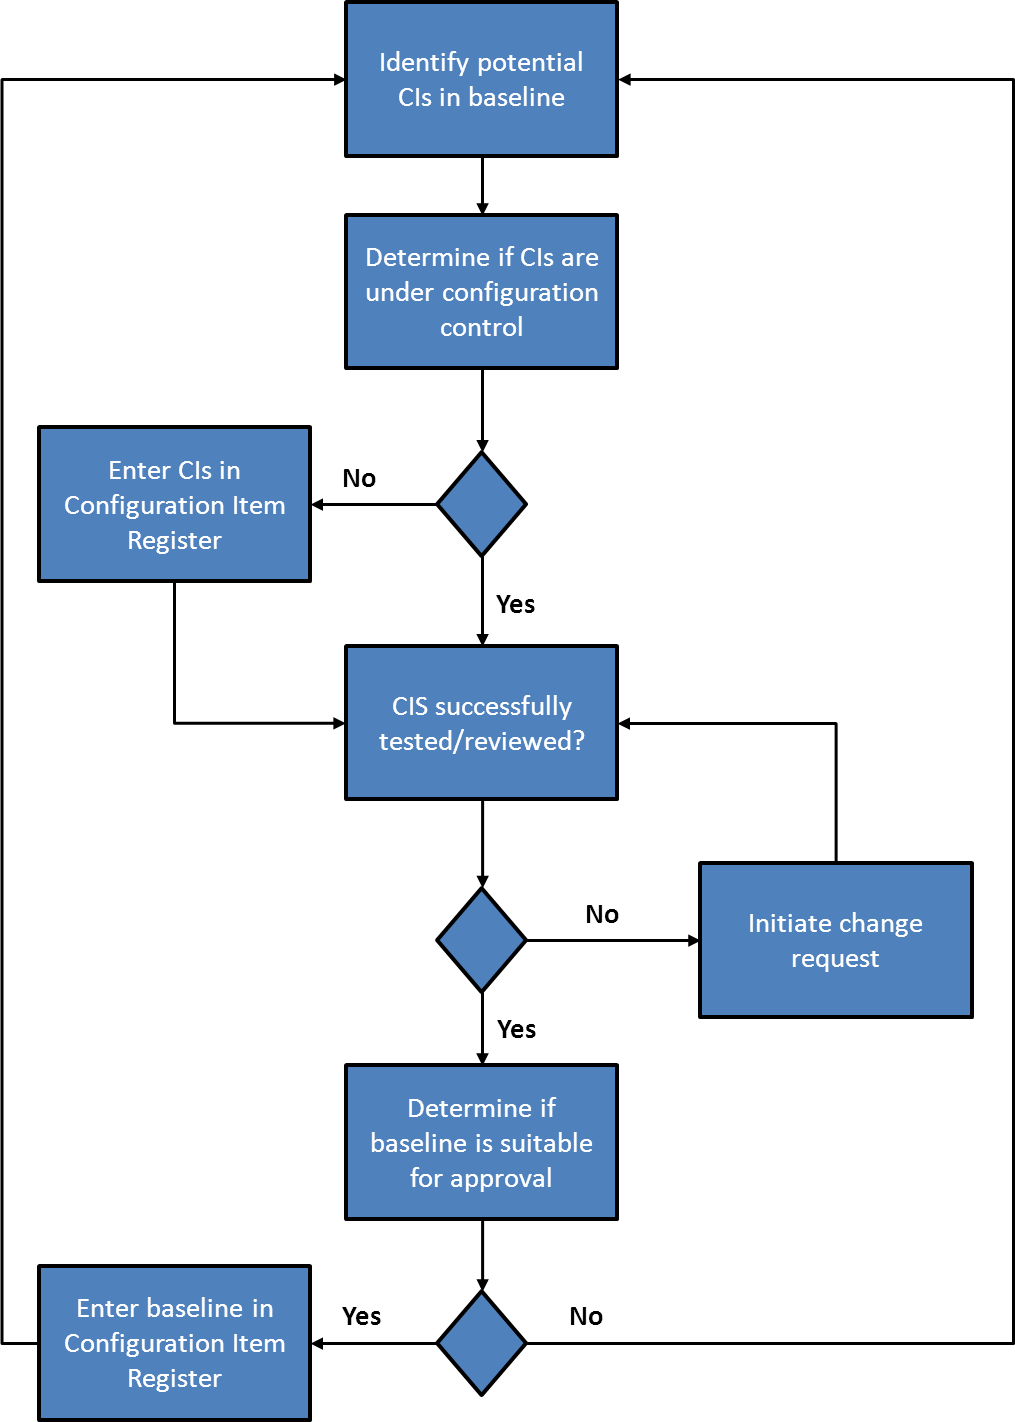
\includegraphics[scale=0.8]{./Figure/Baseline_Process.png}
\end{figure}

Process description:

\vspace{-10pt}
\begin{enumerate}
\item The Work Package Leaders together with the QA Manager and the Configuration Manager are responsible for identifying the CIs that belong to a specific baseline.
\item If a baseline includes a CI that has not been entered into the Configuration Item Register (i.e. placed under configuration control), the CI has to go through the CI identification and selection process (see section \ref{sec:CI Identification and Selection Process}).
\item Before the baseline can be approved, its CIs have to be tested and reviewed individually and as part of the baseline as a whole. If a CI is unsuitable, a change request can be initiated (see section \ref{sec:Configuration Control (Change Management)}).
\item The Work Package Leaders together with the QA Manager and the Configuration Manager decide if the baseline can be approved. If the baseline is approved, the Configuration Item Register is updated accordingly.
\end{enumerate}

\textcolor{red}{Open: Are we tracking baselines through the CI Register?}


\subsection{Configuration Control (Change Management)} % Subsection 3.3
\label{sec:Configuration Control (Change Management)}

Configuration control ensures that CIs are only changed after evaluation and approval. For the openETCS project, a corresponding change management process has been defined separately (see document Change/Problem Management Process in section \ref{sec:References}).


\subsection{Configuration Status Accounting} % Subsection 3.4
\label{sec:Configuration Status Accounting}

Configuration Status Accounting (CSA) is the process of tracking CIs through the steps in their evolution. Regular reports on the status and history of the CIs in the openETCS project are created to deliver the data required to measure project progress. The following data is tracked for each CI:

\textcolor{red}{Open: The QA Plan lists a Software Assessment Plan and Software Assessment Report. Are the requirements below included there, meaning we can simply refer to it here?}

\vspace{-10pt}
\begin{itemize}
\item Approved versions and revisions
\item Status of change requests
\item Implementation status of approved changes
\item Evaluations (Audits)
\end{itemize}

\textcolor{red}{Note: IEEE 828-2005 names the above as the minimum.}

If necessary, this data makes it possible to rebuild previous baselines. It is also used to track change requests and document the results of evaluations and reviews.

\textcolor{red}{Open: The following has to be documented in the SCMP:}

\vspace{-10pt}
\begin{itemize}
\item \textcolor{red}{What data elements and SCM metrics are tracked and reported for baselines and
changes?}
\item \textcolor{red}{What types of status accounting reports are generated (and their frequency)?}
\item \textcolor{red}{How is information collected, stored, processed, reported, and protected from loss?}
\item \textcolor{red}{How is access to the status data is controlled?}
\end{itemize}


\subsection{Configuration Evaluation and Review (Audits)} % Subsection 3.5
\label{sec:Configuration Evaluation and Review (Audits)}

CIs must be evaluated and reviewed (audited) to verify conformance to requirements defined, for example, in the specification documentation of the openETCS project or applicable standards. Audits of CIs must determine that a CI fulfills its required physical and functional characteristics.

\textcolor{red}{Open: The QA Plan lists a Software Verification and Validation Plan (as well as Test, Validation and Verification Reports) and a Software Assessment Plan (and Software Assessment Report). Are those documents going to include the requirements below, meaning we can simply refer to them here?}


\subsubsection{Physical Configuration Audit} % Subsection 3.5.1
\label{sec:Physical Configuration Audit}

A Physical Configuration Audit (PCA) must be carried out prior to a software release or software update (i.e. before a new baseline). It includes all CIs that are part of the corresponding baseline. The PCA is performed to determine that all CIs (including documentation) are present in the correct version and match the data from the corresponding configuration status reports.

An unsuccessful audit (non-conformance) means that the software release or software update cannot take place.

\textcolor{red}{Open: Roles and responsibilities? Process and schedule? Approval criteria and actions that occur upon approval?}


\subsubsection{Functional Configuration Audit} % Subsection 3.5.2
\label{sec:Functional Configuration Audit}

A Functional Configuration Audit (FCA) is carried out for each CI (including documentation) to determine that it has been tested or inspected and fulfills the functions defined in the corresponding openETCS specifications.

An unsuccessful audit (non-conformance) means that the CI cannot be released (e.g. to be part of a baseline).

\textcolor{red}{Open: Roles and responsibilities? Process and schedule? Approval criteria and actions that occur upon approval?}


\subsubsection{Audit Reports} % Subsection 3.5.3
\label{sec:Audit Reports}

Every audit must be documented in a corresponding audit report with at least the following information:

\vspace{-10pt}
\begin{itemize}
\item Auditor
\item Date
\item Audit reason/objective
\item CIs audited
\item Result for each CI
\item Overall result
\item Recipient of audit report
\end{itemize}

\textcolor{red}{Open: Others?}


\subsubsection{Non-Conformance Follow-Up} % Subsection 3.5.4
\label{sec:Non-Conformance Follow-Up}

If a CI fails an audit, corresponding corrective actions have to be planned and implemented before a follow-up audit can be scheduled and carried out. 

\textcolor{red}{Open: Roles and responsibilities? Process?}


\subsection{Interface Control} % Subsection 3.6
\label{sec:Interface Control}

CIs may interface with other items that are outside the scope of the SCMP. The interfacing items may remain outside of configuration control, but the interfaces have to be identified and controlled.

\textcolor{red}{Open: The QA Plan lists a Software Interface Specification. Does that document include the requirements below, meaning we can refer to it here?}

The following information has to be defined for each interface:

\vspace{-10pt}
\begin{itemize}
\item Interface nature/type
\item Affected CIs
\item Process to control interface code, documentation and data
\item Process to approve and release the interface
\end{itemize}

\textcolor{red}{Open: Roles and responsibilities? Process? Do we track/control interfaces as part of individual CIs or as separate items? Is a separate Interface Management Plan planned?}


\subsection{Subcontractor/Vendor Control} % Subsection 3.7
\label{sec:Subcontractor/Vendor Control}

Software items developed outside the openETCS project must be placed under configuration management. This includes software developed by subcontractors or software acquired in finished form form another source. It may not be possible to treat CIs that are not developed internally the exact same way as CIs developed as part of the openETCS project.

If necessary, the following must be determined for subcontractor/vendor CIs:

\vspace{-10pt}
\begin{itemize}
\item SCM requirements the subcontractor has to fulfill
\item Compliance monitoring of the subcontractor
\item Evaluations and reviews of subcontractor CIs
\item Process to test, verify, accept and integrate subcontractor CIs into openETCS project
\item Handling of proprietary CIs (e.g. regarding copyright and royalties)
\item Handling of changes (e.g. participation of subcontractor/vendor)
\end{itemize}

\textcolor{red}{Open: Roles and responsibilities? Process?}


\subsection{Release Management and Delivery} % Subsection 3.8
\label{sec:Release Management and Delivery}

The build, release and delivery of software products and documentation by the openETCS project must be formally controlled. For the openETCS project, a corresponding Software Release and Deployment Plan has been defined separately (see corresponding reference in section \ref{sec:References}).

\newpage


\section{SCM Schedules} % Section 5
\label{sec:SCM Schedules}

Because there may be dependencies between the individual SCM activities or relationships between SCM activities and other project activities (e.g. milestones), some SCM activities  have to be carried out in sequence or according to a schedule.

\textcolor{red}{Open: Do we have dependencies that require sequences/schedules? Are there milestones/events that require SCM activities? Is there some kind of timeline or something we could refer to?}

\newpage


\section{SCM Resources} % Section 5
\label{sec:SCM Resources}

Carrying out the SCM activities defined in this SCMP requires resources. These resources may themselves be CIs that have to be placed under configuration control.

The following table lists the resources specified for each SCM activity:

\begin{center}
\begin{longtable}{m{3cm}m{4cm}m{3cm}m{4cm}}
\caption{SCM resources}\\

\hline \rowcolor{lightgrey} \multicolumn{1}{l}{SCM Activity} & \multicolumn{1}{l}{Tools/Techniques/Equipment} & \multicolumn{1}{l}{Personnel} & \multicolumn{1}{l}{Training} \\ \hline
\endfirsthead

\multicolumn{4}{c}%
{{\bfseries \tablename\ \thetable{} -- continued from previous page}} \\
\hline \rowcolor{lightgrey} \multicolumn{1}{l}{SCM Activity} & \multicolumn{1}{l}{Tools/Techniques/Equipment} & \multicolumn{1}{l}{Personnel} & \multicolumn{1}{l}{Training} \\ \hline
\endhead

\hline \hline
\endlastfoot

CI Identification & & & \\\hline

Baseline Identification & & & \\\hline

Configuration Control & & & \\\hline

Configuration Status Accounting & & & \\\hline

Configuration Evaluation and Review & & & \\\hline

Interface Control & & & \\\hline

Subcontractor/Vendor Control & & & \\\hline

Release Management and Delivery & & & \\\hline

\end{longtable}
\end{center}

\textcolor{red}{Open: Define resources? Can we also refer to corresponding other documents like QA Plan or Change Process?}

\newpage


\section{SCMP Maintenance} % Section 6
\label{sec:SCMP Maintenance}

SCM planning must continue throughout the life cycle of the openETCS project. This means the SCMP itself will be treated as a CI to ensure that the following information remains up-to-date:

\vspace{-10pt}
\begin{itemize}
\item SCM responsibilities
\item SCMP updates (including change management/approval)
\item SCMP distribution
\end{itemize}

\newpage

\bibliography{SCMP_literature_0.0.1}
\bibliographystyle{plain}

\textcolor{red}{Open: Why do we have an additional ''References'' section that basically repeats what is already listed in the ''References, Guidelines and Standards'' section?}


%===================================================
%Do NOT change anything below this line

\end{document}
